\chapter{Architecture et description du logiciel}
Dans cette partie, nous allons d'abord vous parler de la partie concernant le parsing puis passer à la partie d'analyse des données et de rendu graphique.

\section{Architecture globale}

\begin{figure}[!h]
  \begin{center}
    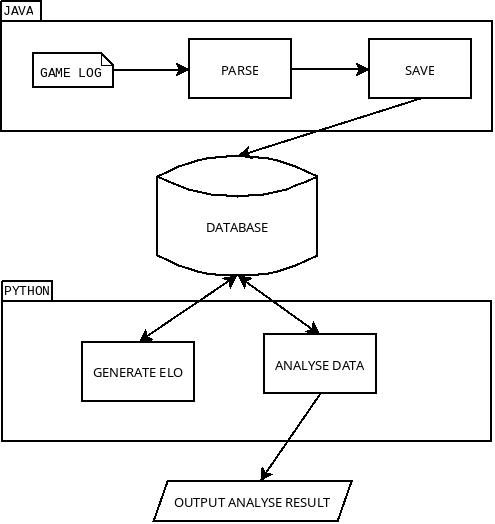
\includegraphics[scale=0.45, keepaspectratio]{./presentation/overview.jpg}
  \end{center}
  \caption{représentation de l'architecture globale du projet}
\end{figure}

L'architecture de notre projet se décompose en 3 parties distinctes et indépendantes. Une première partie permet de charger les données contenues dans les logs puis de les inscrire dans la base de données.\newline
La base de données stocke ces données et peut en recevoir de nouvelles ou bien répondre aux requetes qui lui sont soumises.\newline
La dernière partie correspond à une librairie python permettant à l'utilisateur d'effectuer des analyses prédéfinies ou bien de produire ses propres analyses. Pour cela, l'utilisateur dispose de fonctions de communications avec la base de données.

\section{Partie parser}
Cette partie est écrite en java, l'autre possibilité que nous avions était de coder le parser en python mais après quelques petits tests nous nous sommes rendus compte que le parser en python serait beaucoup trop lent. Voici l'architecture de la partie Java de notre projet:

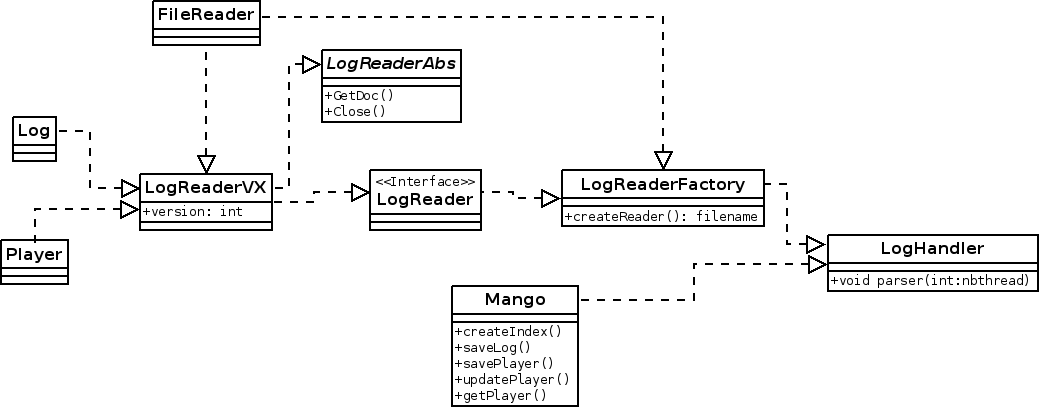
\includegraphics[width=\textwidth,height=\textheight,keepaspectratio]{diaRessources/nouvelleArch}\\

En raison de logs au format variable, il est nécessaire de produire plusieurs versions de parser afin de garder une robustesse au niveau du parsing et d'éviter une classe trop grosse. Pour cela, à l'ouverture d'un log, le LogHandler demande la création d'un parser à une classe utilisant le design pattern factory. Cette classe va examiner le log en question et choisir la bonne version du parser a utiliser puis renvoyer ce parser au log handler. Afin d'éviter des duplications de code inutiles, le parser en lui même est implémenté à l'aide d'une classe abstraite regroupant toutes les similitudes entre les parsers puis les différences sont implémentées dans la classe du parser en question à proprement parler. Le LogHandler va ensuite envoyer sur une base de données les données obtenues à l'aide du parser.

\section{Base de données}
L'implémentation de la base de données retenue est MongoDB, nous l'avons retenue du fait qu'elle soit orientée documents et du fait qu'elle autorise une compression des données stockées. Elle communique avec le parser ainsi que la librairie proposée à l'utilisateur.\\
Elle est capable de recevoir de nouvelles données à stocker, de modifier sa structure (changement ou ajout de champs dans les données) et modifier les données contenues.

\section{Partie Analyse}
Cette partie est écrite en python à la demande du client. Nous avons choisi de proposer plusieurs librairies contenant des outils basiques permettant de travailler sur les données acquises lors du parsing. Voici un schéma regroupant les différentes librairies et leurs liens:

\includegraphics[width=\textwidth,height=\textheight,keepaspectratio]{diaRessources/Python_arch}\\

Tout d'abord, le module MongoInterface permet de communiquer avec la base de données.\newline
Les objets Matchs et Player sont utilisés lors de la récupération de données afin de les mettre en forme pour une utilisation plus aisée par le client. Ce sont des structures de données regroupant toutes les information relatives au match ou joueur en question.\newline
La bilbiothèque Tools regroupe les fonctions d'analyse basique pouvant être utilisées sur les logs, pour appliquer ces fonctions, il faut utiliser la fonction \textit{apply\_function\_to\_query}. Si dans le futur, le client ou bien des personnes souhaitant travailler sur ce projet veulent étoffer les fonctions proposées, il suffira de les ajouter dans cette libraire.\newline
La solution proposée pour afficher les resultats consiste en un module Plotter et un module DataSet. Le module DataSet permet de mettre en forme les données à représenter de manière simple pour l'utilisateur, et le module Plotter propose une solution simple pour afficher des résultats de base (lignes cassées, nuage de points ou barres).

\section{Extensions possibles}
Sur la partie parser, il est très facile d'ajouter une nouvelle version de parser permettant de lire par exemple des logs d'un nouvelle version du serveur de jeu, cela permettrait de regouper des données sur une plus grande période et donc d'obtenir des statistiques plus intéressantes.\newline
Sur la partie Python, il est possible d'ajouter de nouvelles fonctions d'analyse des données, des données peuvent également être rajoutées pour les logs mais il faudra faire attention à la lecture de ces données car les objets ne permettrons pas un accès facile à celles-ci (sauf si l'utilisateur modifie également les structures de données).

\iffalse
Dans cette partie nous cherchons à décrire dans un premier temps [...], puis, c[...].

\section{Partie 1}

Intro

\subsection{Sous-partie 1}

\begin{figure}[!ht]
\begin{center}

\includegraphics[height=12cm]{autre_partie/image1}
\end{center}
\caption[autre partie générale]{autre partie image 1\protect\footnotemark}
%\floatfoot{Source: (Citation command)}
% avec le package "floatrow"
\end{figure}

%footnote protected pour apparaitre dans la légende d'une image
\footnotetext{Schéma d'après : \textit{Auteur 1 \& Propriétaire image}, LICENCE (cf. ref. \cite{cite4})}

\newpage{}

\subsection{Sous-partie 2}

\begin{figure}[!ht]
\begin{center}

\includegraphics[height=12cm]{autre_partie/image2}
\end{center}
\caption[autre partie]{autre partie globale de notre quelque chose}
\end{figure}

Nous retrouvons ici, blabla\footnote{Application bla - Interface blabla} [...].

\subsubsection{Sous-sous-partie 1}

Le bla (cf. ref. \cite{cite6}) est [...]:

\begin{itemize}
\item item1;
\item item2;
\item item3;
\item item4;
\item item5.
\end{itemize}

\newpage

\subsubsection{Sous-sous-partie 2}

%Les lignes :
% \setcounter{secnumdepth}{4}
% \setcounter{tocdepth}{4}
%dans le fichier "main.tex" permettent de faire en sorte que les paragraphes soient interprété comme des titres de niveau 5
\paragraph{Paragraphe 1 (agissant comme titre niveau 5)}
%forcer un saut de ligne
~\\
\hskip7mm

\begin{figure}[!ht]
\begin{center}

\includegraphics[height=6cm]{autre_partie/image3}
\end{center}
\caption[Structure d'unz autre chose]{Structure d'une autre chose\protect\footnotemark}
\end{figure}

Ce schéma représente bla.

\footnotetext{Schéma et explication d'après le wiki bla (cf. ref. \cite{cite0})}

\paragraph{Paragraphe 2}
~\\
\hskip7mm

%fixer les floats précédemment définis
%\FloatBarrier

Bla

\subparagraph{Sous-paragraphe 1}
~\\
\hskip7mm

Bla

\begin{figure}[H]
\begin{center}

\includegraphics[height=10cm]{autre_partie/image4}
\end{center}
\caption{Diagramme de truc}
\end{figure}

\subparagraph{Sous-paragraphe 2}
~\\
\hskip7mm

Bla\\

Bla

\subparagraph{Sous-paragraphe 3}
~\\
\hskip7mm

Bla

\subsubsection{Sous-sous-partie 3}

Bla

\section{Partie 2}

Bla

\footnotetext{D'après le schéma disponible sur la documentfation officielle disponible sur le site blalbla}

Bla

\subsection{Sous-partie 1}

Bla

\subsection{Sous-partie 2}

Bla

\paragraph*{Paragraphe 1 (n'apparaitra pas dans l'index)}
Bla

\paragraph*{Paragraphe 2}
Bla

\paragraph*{Paragraphe 3}
Bla

\subsection{Sous-partie 3}

Bla
\fi
